\documentclass{beamer}
\beamertemplatenavigationsymbolsempty
\usecolortheme{beaver}
\setbeamertemplate{blocks}[rounded=true, shadow=true]
\setbeamertemplate{footline}[page number]
%
\usepackage[utf8]{inputenc}
\usepackage[english]{babel}
\usepackage{amssymb,amsfonts,amsmath,mathtext}
\usepackage[]{algorithmic}
\usepackage{subfig}
\usepackage[all]{xy} % xy package for diagrams
\usepackage{array}
\usepackage{tikz}
\usepackage{multicol}% many columns in slide
\usepackage{hyperref}% urls
\usepackage{hhline}%tables

\newtheorem{hyp}{Hypothesis}


% Your figures are here:
\graphicspath{ {fig/} {../fig/} }

%----------------------------------------------------------------------------------------------------------
\title{Consistency text similarity on the example of the task of recognizing hallucinations of language models}
\author[K. Petrushina]{Kseniia~Petrushina}
\institute{Moscow Institute of Physics and Technology,\\ Skolkovo Institute of Science and Technology}

\date{\footnotesize

\par\smallskip\emph{Scientific supervisor:} Alexander~Panchenko
\par\bigskip\small 2023}
%----------------------------------------------------------------------------------------------------------
\begin{document}
%----------------------------------------------------------------------------------------------------------
\begin{frame}
\thispagestyle{empty}
\maketitle
\end{frame}
%-----------------------------------------------------------------------------------------------------
\begin{frame}{Introduction}
\begin{block}{Explanation}
  \textbf{Hallucination} of the language model is a grammatically correctly generated response, which, however, contains incorrect information.
\end{block}
\begin{block}{Examples}
  Paraphrase generation \& Machine translation -- different meaning.
  Definition modeling -- deviation from the database.
\end{block}
\end{frame}
%-----------------------------------------------------------------------------------------------------

\begin{frame}{Problem statement}

\textit{Language model} is a function 
\[\mathbf{f}: \mathcal{P}(\mathbf{T_s}^{L_s})\to \mathcal{P}(\mathbf{T_h}^{L_h}),\]

$\mathbf{s}_i$ is called \textit{source sentence} and $\mathbf{h}_i$ is called \textit{model hypothesis}.

We can define function \[\mathbf{f}^{-1}: \mathcal{P}(\mathbf{T_h}^{L_h}) \to \mathcal{P}(\mathbf{T_s}^{L_s})\]

Then it is said that $\mathbf{h} = \mathbf{f}(\mathbf{s})$ is a \textit{hallucination} of the language model $\mathbf{f}$ with the input $\mathbf{s}$ if \[p(\mathbf{f}^{-1}(\mathbf{f}(\mathbf{s})) = \mathbf{s}) = 0.\]

\end{frame}
%----------------------------------------------------------------------------------------------------------

\begin{frame}{Problem statement}

The task of recognizing hallucinations is to find a function $sim: \mathbf{T_s}^{L_s} \times \mathbf{T_h}^{L_h} \to [0, 1]$, such that
\[\mathbb{E}_{\mathbf{s}_i \sim \mathbf{T_s}^{L_s}, \mathbf{h}_i \sim f(\mathbf{s}_i)} \{\mathbb{I}[sim(\mathbf{s}_i, \mathbf{h}_i) \ge \text{thr}] = y_i \} \to \max\limits_{sim, \text{thr}},\]
where $y_i$ denotes the presence of a hallucination.

\begin{figure}
    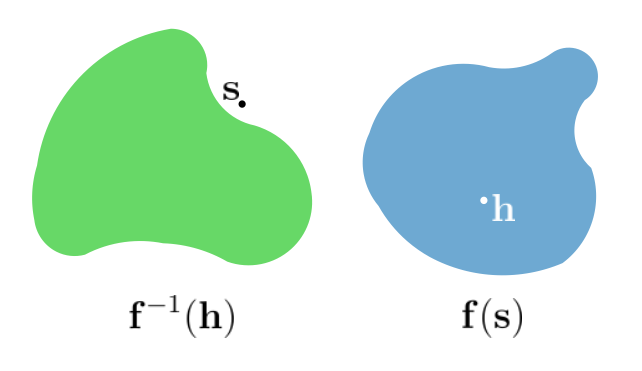
\includegraphics[width=0.4\textwidth]{images/hallucination.png}
    \caption{An illustration of a model's hallucination. $\mathbf{s}$ does not belong to the set of possible outputs of $\mathbf{f}^{-1}(\mathbf{h})$}
    \label{fig:hal}
\end{figure}


\end{frame}
%----------------------------------------------------------------------------------------------------------

\begin{frame}{Existing solutions}

\begin{enumerate}
    \item \textbf{Words or characters n-grams} \[sim_\text{BLEU}(\mathbf{s}, \mathbf{h}) = \frac{|N_{s} \cap N_{h}|}{|N_{h}|}\]
    \item \textbf{Similarity between static embeddings} \[sim_\text{cos}(\mathbf{s}, \mathbf{h}) = \cos (\mathbf{v_s}, \mathbf{v_h})\]
    \item \textbf{Similarity between contextualized embeddings} \[R = \dfrac{1}{L_s} \sum\limits_{v_i \in \mathbf{v_s}} \max\limits_{\hat{v}_j \in \mathbf{v_h}} v^T_i \hat{v}_j \; P = \dfrac{1}{L_h} \sum\limits_{\hat{v}_j \in \mathbf{v_h}} \max\limits_{v_i \in \mathbf{v_s}} v^T_i \hat{v}_j \] 
    \[\text{BERTScore} = 2\dfrac{P R}{P + R}\]
\end{enumerate}

\end{frame}
%----------------------------------------------------------------------------------------------------------

\begin{frame}{Existing solutions}

\begin{enumerate}
    \item[4.] \textbf{Similarity between embeddings from bi-encoders} \[sim_\text{bi-enc}(\mathbf{s}, \mathbf{h}) = \cos (\mathbf{enc_s}(\mathbf{s}), \mathbf{enc_h}(\mathbf{h}))\]
    \item[5.] \textbf{Symmetric and asymmetric cross-encoders} \[sim_\text{cross-enc}(\mathbf{s}, \mathbf{h}) = \mathbf{clf}(\mathbf{enc}(\mathbf{s}, \mathbf{h}))\]
\end{enumerate}

In the general case, the similarity function should be defined for objects from different spaces $\mathbf{T_s}^{L_s}$ and $\mathbf{T_h}^{L_h}$. 

The existing methods do not investigate whether there is enough information in $\mathbf{h}$ to restore $\mathbf{s}$.

\end{frame}
%----------------------------------------------------------------------------------------------------------

\begin{frame}{Consistency similarity}


Consistency similarity measure is defined by
\[{sim}_{\mathbf{C}} (\mathbf{s}_i, \mathbf{h}_i) = {sim}(\mathbf{s}_i, \mathbf{f}^{-1}(\mathbf{h}_i))).\]

\begin{enumerate}
    \item The arguments of the function lie in the same space $\mathbf{T_S}^{L_s}$.
    \item This similarity measure depends on how well the information about $\mathbf{s}_i$ is preserved in $\mathbf{h}_i$ and what the model $\mathbf{f}^{-1}$ can restore.
\end{enumerate}

\begin{hyp}
\begin{enumerate}
    \item \[\mathbb{E}_{\mathbf{f}^{-1}(\mathbf{h}_i)} {sim}_{\mathbf{C}} (\mathbf{s}_i, \mathbf{h}_i) \le{sim} (\mathbf{s}_i, \mathbf{h}_i) \]
    \item \[\mathbb{E}_{\mathbf{s}_i \sim \mathbf{T_s}^{L_s}, \mathbf{h}_i \sim f(\mathbf{s}_i)} \{\mathbb{I}[sim_\text{C}(\mathbf{s}_i, \mathbf{h}_i) \ge \text{thr}] = y_i \} \ge \]
    \[\mathbb{E}_{\mathbf{s}_i \sim \mathbf{T_s}^{L_s}, \mathbf{h}_i \sim f(\mathbf{s}_i)} \{\mathbb{I}[sim(\mathbf{s}_i, \mathbf{h}_i) \ge \text{thr}] = y_i \}\]
\end{enumerate}    
\end{hyp}

\end{frame}
%----------------------------------------------------------------------------------------------------------

\begin{frame}{Computational experiment}

\subsection{Data}

We are given the dataset
\[\mathcal{D} = \{(\mathbf{s}_i, \mathbf{h}_i, y_i) \}_{i=1}^N, \quad \mathbf{h}_i \in \mathbf{f}(\mathbf{s}_i), \quad y_i \in \{0, 1\}\]

The target variable $y_i$ indicates the occurrence of a hallucination in the $\mathbf{f}$ model at the input of $\mathbf{s}_i$ and the output of $\mathbf{h}_i$.

\subsection{Metrics}

\begin{enumerate}
    \item The proportion of correct predictions:
    \[\text{Accuracy} = \frac1N \sum\limits_{i=1}^N \mathbb{I}[\hat{y}_i \ge \text{thr}] = y_i\]
    \item Spearman's rank correlation coefficient:
    \[r_s= \rho_{R(Y), R(\hat{Y})} = \frac{\text{cov} (R(Y), R(\hat{Y}))}{\sigma_{R(Y)} \sigma_{R(\hat{Y})}}\]
\end{enumerate}


\end{frame}
%----------------------------------------------------------------------------------------------------------

\begin{frame}{Results}

\begin{itemize}
    \item Paraphrase generation task\\
    \begin{table}[]
        \centering
        \begin{tabular}{c|c c}
        Method & Accuracy $\uparrow$ & $r_s \uparrow$ \\
        \hline
        $sim_\text{bi-enc}$ & 0.808 & 0.153 \\
        $sim_\text{C}$ & \textbf{0.824} & \textbf{0.186} \\
        \end{tabular}
        \caption{Hallucination recognition results in the PG task}
        \label{tab:pg}
    \end{table}
    \item Machine translation task\\

    \begin{table}[]
    \centering
    \begin{tabular}{c|c c}
    Method & Accuracy $\uparrow$ & $r_s \uparrow$ \\
    \hline
    $sim_\text{LaBSE}$ & 0.786 & 0.592 \\
    $sim_\text{BLASER-QE}$ & \textbf{0.802} & \textbf{0.605} \\
    \end{tabular}
    \caption{Hallucination recognition results in the MT task}
    \label{tab:mt}
    \end{table}

\end{itemize}


\end{frame}
%----------------------------------------------------------------------------------------------------------

%----------------------------------------------------------------------------------------------------------
\begin{frame}{Conclusion}
  \begin{itemize}
      \item Analysis of the existing measures of textual similarity.
      \item New method that corrects the disadvantages of the previous ones.
      \item Hypotheses about properties of the \textit{consistency similarity measure}.
      \item Computational experiments with different measures.
  \end{itemize}

  \textbf{Future work}: 
  \begin{itemize}
      \item Theoretical justification of hypotheses.
      \item Extend the method to work with an external database
      \item Conduct comprehensive ablation study.
  \end{itemize}
\end{frame}
%----------------------------------------------------------------------------------------------------------

\begin{frame}{Literature}
\begin{enumerate}
    \item David Dale et al. 2023. \textcolor{blue}{HalOmi: A Manually Annotated Benchmark for Multilingual Hallucination and Omission Detection in Machine Translation}.
    
    URL: \url{https://arxiv.org/pdf/2305.11746.pdf}

    \item Nikolay Babakov et al. 2022. \textcolor{blue}{A large-scale computational study of content preservation measures for text style transfer and paraphrase generation}. %In Proceedings of the 60th Annual Meeting of the Association for Computational Linguistics: Student Research Workshop, pages 300–321, Dublin, Ireland. Association for Computational Linguistics.

    URL: \url{https://aclanthology.org/2022.acl-srw.23.pdf}

    \item Ashish Vaswani et al. 2017. \textcolor{blue}{Attention is All you Need}

    URL: \url{https://proceedings.neurips.cc/paper_files/paper/2017/file/3f5ee243547dee91fbd053c1c4a845aa-Paper.pdf}
    


  \end{enumerate}
\end{frame}
\end{document} 
